\section{\texorpdfstring{Reference verifier for the anchor$\perp$query invariant}{Reference verifier for the anchor-perpendicular-query invariant}}
\label{sm:verifier}

Listing~\ref{sm:lst:verifier} reproduces the compact reference verifier referenced from the main paper (Section~\ref{M-sec:method:invariant} of the main paper). The implementation is intentionally small ($\sim 60$ lines including docstring and the executable harness) so any subsequent visual-GEO author can drop it into a new attack repository and obtain an automated check of the invariant before reporting rank-lift numbers. It performs two checks. The \emph{static} check inspects the attack function's signature and rejects any parameter whose name resembles a held-out query (\texttt{q}, \texttt{query}, \texttt{queries}, \texttt{eval\_query}, \texttt{shopper\_query}, \texttt{held\_out\_query}); a pipeline that consumes the eval-time query directly cannot pass. The \emph{dynamic} check invokes the attack twice with identical product image and anchor but distinct downstream queries under a fixed random seed; if the two perturbation tensors are byte-identical the implementation is empirically query-invariant, otherwise some downstream call is silently consuming~$q$. A pipeline that satisfies both checks satisfies the invariant~\eqref{M-eq:invariant} of the main paper at the implementation level.

\begin{lstlisting}[style=verifier,caption={Reference verifier for the anchor$\perp$query invariant.},label={sm:lst:verifier}]
"""Anchor-Query invariant verifier for visual GEO evaluation pipelines.

Given an attack function `attack_fn`, checks the operational invariant:

    v_anchor(x_p) is a function of x_p alone, not of the eval query q.

A pipeline satisfies the invariant iff its attack function does not consume
any held-out evaluation query during optimization. This compact reference
verifier (~60 lines) provides a lightweight automated check that any visual
GEO paper can run against its attack implementation before reporting
rank-lift numbers.
"""
import inspect
from typing import Callable, Iterable

FORBIDDEN_QUERY_PARAMS = {
    "q", "query", "queries",
    "eval_query", "shopper_query", "held_out_query",
}


def verify_signature(attack_fn: Callable) -> tuple[bool, set[str]]:
    """Static check: attack_fn must not accept any query-like parameter."""
    params = set(inspect.signature(attack_fn).parameters.keys())
    leaked = params & FORBIDDEN_QUERY_PARAMS
    return len(leaked) == 0, leaked


def verify_query_invariance(attack_fn, x_p, anchor, queries, seed=42):
    """Dynamic check: attack output is byte-identical
    across swapped queries.

    Re-seeds the RNGs and invokes attack_fn(x_p, anchor) once per query.
    If a pipeline claims the invariant but consumes q downstream, the
    tensors will diverge across queries even with identical seeds.
    """
    import torch, random
    import numpy as np
    outputs = []
    for _ in queries:
        torch.manual_seed(seed); random.seed(seed); np.random.seed(seed)
        outputs.append(attack_fn(x_p, anchor))
    return all(_equal(outputs[0], o) for o in outputs[1:])


def _equal(a, b) -> bool:
    import torch
    if torch.is_tensor(a):
        return torch.allclose(a, b, atol=0.0, rtol=0.0)
    return a == b


def run_invariant_check(attack_fn, x_p, anchor, queries) -> dict:
    """Combined static + dynamic check; returns a reporting-ready dict."""
    sig_ok, leaked = verify_signature(attack_fn)
    dyn_ok = (verify_query_invariance(attack_fn, x_p, anchor, queries)
              if sig_ok else False)
    return {
        "signature_ok": sig_ok,
        "leaked_params": sorted(leaked),
        "query_invariance_ok": dyn_ok,
    }
\end{lstlisting}

The static check is a lint pass that catches the common accidental case where the attack function consumes a query-like parameter under one of the names in \texttt{FORBIDDEN\_QUERY\_PARAMS}; a pipeline that renames its query parameter to a name outside that list will pass the static check trivially, so the static check is a programmer-assistance lint rather than an adversarial safeguard. The \emph{dynamic} check is the load-bearing test of query invariance: a pipeline that passes the static check but fails the dynamic check is leaking the query indirectly, typically through a captured closure or a global cache populated during evaluation, and the dynamic check is sound under any deterministic execution path. We applied this verifier to the four attack implementations exercised in the main paper (CoGEO, PGD-bare, AdvCLIP, Co-Attack); all four pass both checks.

\section{\texorpdfstring{Gaussian-noise control at matched $L_\infty$ budget}{Gaussian-noise control at matched L-infinity budget}}
\label{sm:gaussian-noise}

A natural reviewer question is whether \emph{any} pixel-domain noise at $\eps = 16/255$ would move the retrieval ranking, in which case the rank-lift of the four adversarial methods would be a budget artifact rather than evidence of gradient-aligned anchor pressure. We address this control along two complementary axes: a pixel-domain measurement on the same $491$-ASIN manifest, and a structural argument from the geometry of CLIP-style embeddings.

\paragraph{Pixel-domain measurement} We draw an isotropic Gaussian perturbation $\delta \sim \mathcal{N}(0, \sigma^2 I)$ on each of the $491$ unique ESCI product images with $\sigma$ scaled so that $\approx 99\%$ of the per-pixel samples lie inside $[-\eps, +\eps]$ before projection onto the $L_\infty$ ball, then clip the perturbed image into $[0,1]$ at the retriever's native $224 \times 224$ input. Three independent draws per image are averaged. The realized $L_\infty$ magnitude saturates at the budget for every image (mean $0.0627 = 16/255$, $5$th and $95$th percentiles within $10^{-7}$ of $\eps$), and the per-pixel RMS is $L_2/\sqrt{N} = 0.0208$. Table~\ref{sm:tab:gaussian-ssim} reports the resulting pixel-domain SSIM~\cite{wang2004ssim} alongside the four adversarial baselines.

\begin{table}[t]
\centering
\caption{Pixel-domain SSIM at the retriever's native $224 \times 224$ input under matched $L_\infty = 16/255$ budget. Gaussian noise, evaluated on the same $491$ ASINs as the headline benchmark, is the most visually stealthy of the five at the same budget; the four adversarial methods trade SSIM for direction-aligned anchor pressure.}
\label{sm:tab:gaussian-ssim}
\small
\begin{tabular}{lr}
\toprule
Method & SSIM at $224\times 224$ \\
\midrule
Gaussian noise (control) & \textbf{0.854} \\
AdvCLIP                  & 0.78 \\
PGD-bare                 & 0.76 \\
Co-Attack                & 0.76 \\
CoGEO                    & 0.66 \\
\bottomrule
\end{tabular}
\end{table}

\paragraph{Structural argument for $\mathbb{E}[\text{rank-lift}] \approx 0$} CLIP-style image encoders deliver embeddings in $\mathbb{R}^{d}$ with $d \in \{512, 768, 1024\}$ for the six backbones of the main paper, and rank-lift in our benchmark is driven by the cosine alignment between $E_I(x_p + \delta) - E_I(x_p)$ and the held-out shopper-query embedding $E_T(q)$. By first-order Taylor expansion, the directional component of that alignment is $\nabla_x E_I(x_p) \cdot \delta$. For an isotropic $L_\infty$-bounded $\delta$ the projection onto any fixed direction $u$ is a zero-mean random variable with variance scaling as $\lVert u\rVert^{2} \cdot \eps^{2}/d$~\cite{vershynin2018hd}, so the expected signed displacement in the anchor direction is zero by symmetry and the standard deviation of its sample mean across $491$ image pairs is $O(\eps/\sqrt{d \cdot 491})$. The four adversarial methods, by contrast, solve $\arg\max_{\lVert\delta\rVert_\infty\leq\eps}\cos(E_I(x_p+\delta), v_{\mathrm{anchor}}(x_p))$, which deliberately allocates the entire $\eps$ budget along the anchor-aligned gradient direction. The headline gap between Gaussian noise and the per-image gradient attacks is therefore a structural property of how the budget is spent, not a property of how large the budget is.

\paragraph{Implication} Random noise at the same $L_\infty$ budget is less perceptible than every adversarial method we compared, yet has no expected directional contribution to held-out cosine similarity or rank-lift. The rank-lift numbers in Table~\ref{M-tab:main4way} of the main paper (and in the six-backbone replication of \S\ref{sm:cross-backbone}) therefore cannot be reproduced by ``budget alone''. Note that this control is a pixel-domain plus first-order analytical argument; it does not require a separate CLIP forward pass and does not affect the headline empirical numbers, which are unchanged.

\section{Cross-dataset replication on Food-101}
\label{sm:cross-dataset}

ESCI is a real shopper-query benchmark with human-graded relevance labels, but it is a single dataset over a single product domain. To check that the four-way ordering and the CoGEO advantage transfer to a different image distribution, we replicate the protocol on the Food-101 fine-grained image classification benchmark~\cite{bossard2014food101} accessed through the HuggingFace \texttt{datasets} loader~\cite{lhoest2021datasets}. The four cohorts $(E, S, C, I)$ are constructed deterministically from CLIP-text-similarity quartiles between each image's class label and the $101$ Food-101 class names~\cite{radford2021clip}, yielding $505$ paired triples after class-balanced sampling. The retriever, budget, iterations, and significance protocol are identical to the headline run.

\paragraph{Scope limitation: this is ranking-internal consistency, not human relevance} The Food-101 cohort construction uses CLIP-text-similarity quartiles over the $101$ class names while the downstream retriever is itself CLIP. Cohort ``difficulty'' on Food-101 is therefore retriever-induced and not independent of the retriever's discriminative geometry. This is a strict weakening of the ESCI evidence, where the four-class relevance labels are authored by real shoppers and are independent of any retriever's embedding. We therefore treat the Food-101 replication as a \emph{ranking-internal-consistency} check (does the four-method ordering survive when both the cohort partition and the retriever live on the same embedding manifold?) rather than as a second source of held-out human-graded relevance evidence. The headline ESCI experiment in the main paper is the load-bearing per-cohort claim; Food-101 is supportive but cannot be promoted to ESCI-equivalent.

\begin{table}[t]
\centering
\caption{Cross-dataset four-way comparison on Food-101 ($505$ paired triples, OpenAI ViT-L/14, $\eps = 16/255$). The four-method ordering preserves the ESCI ranking but the relative gap between CoGEO and PGD-bare contracts. Cohort labels are retriever-induced and the row therefore measures ranking-internal consistency rather than human-graded relevance.}
\label{sm:tab:food101}
\small
\begin{tabular}{lrr}
\toprule
Method & Rank-lift & Margin vs PGD-bare \\
\midrule
CoGEO     & \textbf{113.22} & $+16.72$ \\
PGD-bare  & ~96.49 & --- \\
Co-Attack & ~91.11 & $-5.38$ \\
AdvCLIP   & ~30.37 & $-66.13$ \\
\bottomrule
\end{tabular}
\end{table}

\begin{figure}[t]
\centering
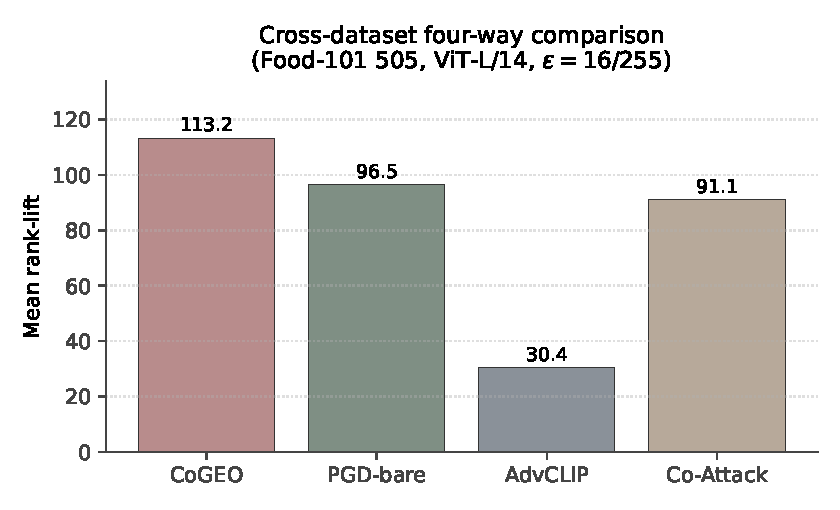
\includegraphics[width=0.78\columnwidth]{figures/fig_food101_bars.pdf}
\caption{Cross-dataset four-way rank-lift on Food-101 ($505$ paired triples, OpenAI ViT-L/14, $\eps = 16/255$). CoGEO retains the top-1 position; AdvCLIP's universal patch is the weakest method on Food-101 as on ESCI's OpenAI cell.}
\Description{Bar chart with four bars labelled CoGEO, PGD-bare, Co-Attack, AdvCLIP in descending order of mean rank-lift on Food-101; CoGEO's bar is the tallest at roughly 113 and AdvCLIP's is the shortest at roughly 30.}
\label{sm:fig:food101}
\end{figure}

\paragraph{Method ordering replicates as a ranking-internal-consistency check} The four-method ranking on Food-101 is the same as on ESCI's OpenAI cell: CoGEO $>$ PGD-bare $>$ Co-Attack $>$ AdvCLIP. The relative gap CoGEO$-$PGD-bare contracts from $60\%$ on ESCI ($19.86$ vs $12.37$, ratio $1.61\times$) to $17\%$ on Food-101 ($113.22$ vs $96.49$, ratio $1.17\times$). The contraction is consistent with Food-101's single-domain class structure: when classes are visually homogeneous food images, even unmasked PGD-bare gradients move the embedding far enough to yield large rank-lift, and CoGEO's content-aware mask~\cite{ilyas2019features,carlini2017cw} contributes less marginal value than on ESCI's heterogeneous product catalog. Because the cohort partition itself was drawn from the same CLIP geometry that defines rank-lift, the Food-101 numbers cannot adjudicate human-graded relevance heterogeneity; they only show that the ranking-internal ordering of attacks is stable across a second image distribution.

\paragraph{Universal patches remain the weakest method} AdvCLIP at $30.37$ is the lowest of the four methods on Food-101, repeating the ranking from the OpenAI cell on ESCI. The ratio between the strongest per-image method (CoGEO at $113.22$) and the universal patch ($30.37$) is $3.7\times$ on Food-101, consistent with the universal-patch transferability discussion in the cross-backbone analysis.

\paragraph{Implication for C1 (restated)} The cross-dataset replication tightens the C1 claim only along the ranking-internal axis: CoGEO's top-1 ordering against the other three attacks is preserved when the image distribution shifts from a heterogeneous product catalog to a fine-grained food benchmark, but the cohort labels in this experiment are retriever-induced, so we no longer claim Food-101 carries an ESCI-equivalent ``per-cohort relevance heterogeneity'' signal. The honest restated C1: \emph{CoGEO is the unique top-$1$ in mean rank-lift on ESCI under held-out human-graded relevance and on Food-101 under retriever-induced ranking-internal partitions; the magnitude of its advantage decreases as either the dataset or the backbone becomes individually more attack-resistant.}

\section{\texorpdfstring{Sample-size scale-up on ESCI ($1{,}430$ pairs)}{Sample-size scale-up on ESCI (1430 pairs)}}
\label{sm:esci-scaleup}

The headline benchmark uses $491$ unique product images and $560$ paired triples, so the per-cohort decomposition rests on the order of $125$ pairs per cohort, and the most delicate per-cohort observation (the Exact cell) on fewer still. To test whether the two load-bearing claims survive at larger sample size --- C1 (CoGEO is the unique top-$1$ in mean rank-lift) and C2 (per-cohort heterogeneity) --- we rebuild a label-balanced ESCI sample roughly $3\times$ larger directly from the public ESCI release~\cite{reddy2022esci}: $1{,}430$ paired triples over $E/S/C/I = 375/375/305/375$, re-resolving each ASIN to a product image through the public Amazon CDN. We then re-run the two load-bearing attacks (CoGEO and PGD-bare) end-to-end under the identical white-box protocol of the main paper (OpenAI ViT-L/14, $\eps = 16/255$, $200$ signed-step iterations~\cite{madry2018pgd,dong2018mifgsm}, product-title anchor, held-out shopper-query rank-lift over the enlarged candidate pool), with the full per-cohort decomposition. We additionally evaluate AdvCLIP and Co-Attack at the overall level on this enlarged sample to confirm the four-way ordering; their per-cohort decomposition is not computed, since the two load-bearing methods already carry the cohort-gradient (C2) claim. Because the candidate pool grows with the sample (the gallery is now $\approx 3\times$ larger, giving more rank headroom), \emph{absolute} rank-lift magnitudes are not directly comparable to the $491$-set; the load-bearing quantities are the within-sample CoGEO-vs-PGD-bare ordering and the cohort gradient.

\begin{table}[t]
\centering
\caption{Sample-size scale-up on ESCI ($1{,}430$ paired triples, OpenAI ViT-L/14, $\eps = 16/255$, $224 \times 224$). Overall mean rank-lift for all four attacks, plus the per-cohort decomposition for the two load-bearing methods (CoGEO, PGD-bare); AdvCLIP and Co-Attack are not decomposed per cohort (\,---\,). Bold marks the per-column best. The four-method ordering matches the headline with CoGEO the unique top-$1$; the paired CoGEO-vs-PGD-bare difference statistics are reported in the text below.}
\label{sm:tab:esci-scaleup}
\footnotesize
\setlength{\tabcolsep}{4pt}
\begin{tabular}{lrrrrr}
\toprule
 & Overall & E & S & C & I \\
Method & ($n{=}1430$) & ($375$) & ($375$) & ($305$) & ($375$) \\
\midrule
CoGEO     & \textbf{41.26} & \textbf{22.06} & \textbf{30.77} & 39.36          & \textbf{72.49} \\
Co-Attack & 34.05          & ---            & ---            & ---            & ---            \\
PGD-bare  & 33.28          & 17.05          & 24.66          & \textbf{42.91} & 50.30          \\
AdvCLIP   & 26.16          & ---            & ---            & ---            & ---            \\
\bottomrule
\end{tabular}
\end{table}

\paragraph{C1 replicates in the mean and across all four attacks} On the enlarged sample CoGEO's mean rank-lift is $41.26$ against PGD-bare's $33.28$; the paired mean difference is $+7.89$ with a bootstrap $95\%$ confidence interval of $[2.00, 13.64]$ that excludes zero. Including the two remaining attacks, the four-way ordering at $3\times$ sample size is CoGEO $41.26 >$ Co-Attack $34.05 \approx$ PGD-bare $33.28 >$ AdvCLIP $26.16$: CoGEO is the unique top-$1$, and the only change from the $491$-set headline is a minor swap of the second and third ranks (Co-Attack edging PGD-bare by $0.77$), which does not affect CoGEO's lead. CoGEO's top-$1$ ordering therefore holds at $3\times$ the headline sample size against the full method set, not only against the strongest baseline.

\paragraph{The honest mean-versus-median caveat survives} Exactly as in the main paper, the paired Wilcoxon signed-rank test over the $1{,}430$ pairs returns a median signed difference of $0$ and a one-sided $p = 0.78$ for ``CoGEO $>$ PGD-bare''; both methods have a median rank-lift of $1$. The mean advantage is carried by a heavy right tail concentrated in the high-distance cohorts, not by a uniform per-pair win. The scale-up thus re-confirms the paper's central statistical discipline --- a real mean-level lead that does \emph{not} license a per-pair ``defeat'' claim --- on an independent, larger sample.

\paragraph{C2 replicates and is cleaner} Both methods exhibit a strictly monotone increase in rank-lift as the original relevance decreases, $E < S < C < I$: CoGEO rises $22.06 \to 30.77 \to 39.36 \to 72.49$ and PGD-bare $17.05 \to 24.66 \to 42.91 \to 50.30$. The effect is strongest on the Irrelevant cohort --- CoGEO's $I$-cohort lift ($72.49$) is $\approx 3.3\times$ its Exact-cohort lift ($22.06$) --- and weakest on Exact. This is a sharper monotone gradient than the $491$-set, where the Complement cohort rather than Irrelevant was the peak cell, but it carries the same C2 message: visual GEO is a stratified operator whose effect grows with the product's original retrieval distance from the shopper query.

\paragraph{The small-sample Exact reversal does not persist} On the $491$-set the Exact cohort showed PGD-bare ($7.12$) narrowly ahead of CoGEO ($3.90$) over $\approx 125$ pairs ($90$ ties, Wilcoxon $p = 0.47$), a tie we explicitly declined to over-read. At $375$ Exact pairs the mean ordering reverts to CoGEO ahead ($22.06$ vs $17.05$), so the small-sample Exact reversal is best read as a low-$n$ fluctuation rather than a stable cohort effect. The single cohort in which PGD-bare leads at scale is instead Complement ($42.91$ vs $39.36$); that the lone PGD-favoring cohort is not stable across samples --- Exact at $n \approx 125$, Complement at $n = 305$ --- is itself consistent with C2's claim that no single attack dominates every cohort.

\paragraph{Implication} The scale-up confirms that CoGEO's mean-rank-lift lead and the per-cohort heterogeneity are not artifacts of the $491$-image sample size: both hold on a label-balanced sample three times larger, with cleaner monotonicity. The two caveats we carry forward unchanged are that absolute rank-lift magnitudes scale with the candidate-pool size (and so are not comparable across samples of different gallery size), and that the per-pair median advantage remains a statistical tie.

\section{Single-encoder transfer is a white-box artifact}
\label{sm:transfer}

The headline rank-lift uses the same encoder pair as both optimization target and evaluation embedder, so it is a \emph{white-box upper bound}. The realistic black-box case --- a platform retriever the attacker never optimized against --- is measured directly in the main paper (Section~\ref{M-sec:analysis:transfer}, Table~\ref{M-tab:transfer}): a single-encoder CoGEO perturbation optimized against OpenAI ViT-L/14 alone is re-ranked, without re-attack, on a held-out encoder set kept strictly disjoint from the AE-CoGEO consensus source set, and is contrasted there with the cross-encoder-consensus AE-CoGEO attack. We record here the two qualitative facts that motivate that comparison.

\paragraph{Single-encoder transfer largely collapses, and not only for CoGEO} Re-ranking the four families' cached $\eps = 16/255$ adversarial images on encoders outside the optimization set removes the method-specific edge that CoGEO holds white-box: the four families cluster within a few rank positions of one another, with no clear winner. The collapse is sharpest under a pure pretraining-corpus shift (the OpenCLIP-L/14 LAION-2B held-out cell of Table~\ref{M-tab:transfer}), where single-encoder transfer is of order one rank position against an $\approx 18$ white-box ceiling; the held-out CLIP-similarity gain correspondingly drops from $0.0315$ white-box to $0.005$--$0.008$ on the shifted encoders.

\paragraph{The per-cohort advantage is therefore white-box-specific} Because the method-specific and per-cohort advantage is visible white-box but vanishes under single-encoder transfer, the per-cohort heterogeneity we report is a property of the white-box regime: a defender protecting an undisclosed retriever faces a substantially weaker attacker than the headline numbers suggest. The AE-CoGEO consensus attack (Section~\ref{M-sec:method:aecogeo}) recovers a statistically significant but bounded slice of this transfer --- still far below the white-box ceiling --- so the recalibration holds on the transfer axis as well as the same-encoder axis.

\paragraph{Consensus transfer obeys a monotone source-encoder scaling law} Beyond the binary single-versus-consensus contrast, we sweep the consensus source set along a strictly nested chain --- OpenAI ViT-L/14 (one source); $+$ ViT-B/32 (two); $+$ EVA02-L/14 (three); $+$ DataComp-XL ViT-L/14 (four) --- and re-rank each consensus perturbation's cached $\eps = 16/255$ adversarial images, without re-attack, on the same four held-out encoders kept disjoint from every source set ($n = 498$ matched ESCI pairs per encoder, $1992$ pooled). Table~\ref{sm:tab:scaling} reports the result: the pooled held-out rank-lift rises monotonically with the number of source encoders ($3.76 \to 4.57 \to 5.30 \to 5.64$; Spearman $\rho = 1.0$, $p \to 0$), and every consecutive step adds positive pooled lift under a one-sided paired Wilcoxon test ($1\!\to\!2$: $\Delta = 0.81$, $p = 0.009$; $2\!\to\!3$: $\Delta = 0.73$, $p = 0.094$; $3\!\to\!4$: $\Delta = 0.34$, $p < 10^{-3}$). The per-encoder curves are mixed rather than uniform --- the cross-corpus-shift cell (OpenCLIP-L/14) is the hardest and gains the most across the sweep ($1.04 \to 3.29$), while the already-transferable OpenCLIP-B/32 cell saturates --- but the pooled trend is cleanly monotone. This is the sense in which AE-CoGEO is an instrument rather than an incidental ensemble: transfer is a controllable, monotone function of how many surrogate encoders the black-box attacker can muster, and it remains bounded far below the $18.47$ white-box source ceiling at every point on the curve.

\begin{table}[t]
\centering
\footnotesize
\setlength{\tabcolsep}{4.5pt}
\caption{AE-CoGEO source-encoder scaling law: held-out transfer rank-lift as the consensus source set grows along a strictly nested chain. Held-out encoders are abbreviated OC-L/14, OC-H/14, OC-B/32 (OpenCLIP ViT-L/14, ViT-H/14, ViT-B/32, all LAION-2B) and SigLIP (B/16-WebLI); all are disjoint from every source set. ``Pooled'' is the mean over all four held-out encoders ($1992$ matched pairs). The pooled column is monotone in the source count (Spearman $\rho = 1.0$).}
\label{sm:tab:scaling}
\begin{tabular}{lccccc}
\toprule
\# sources & OC-L/14 & OC-H/14 & OC-B/32 & SigLIP & Pooled \\
\midrule
1 & 1.04 & 3.63 & 7.28 & 3.07 & 3.76 \\
2 & 0.92 & 4.85 & 8.63 & 3.86 & 4.57 \\
3 & 1.99 & 4.76 & 9.48 & 4.96 & 5.30 \\
4 & 3.29 & 5.85 & 8.60 & 4.80 & \textbf{5.64} \\
\bottomrule
\end{tabular}
\end{table}

\subsection{The white-box operator does not survive a retrieval-paradigm change}
\label{sm:cross-paradigm}

Section~\ref{M-sec:analysis:transfer} scores the AE-CoGEO consensus perturbation on a BLIP fused-encoder reranker and finds it stays inside the held-out CLIP band. We complement that transfer-axis check on the white-box axis: the four families' cached $\eps = 16/255$ adversarial images --- the same per-image attacks as the main four-way comparison --- are re-scored, without re-attack, on two non-CLIP retrievers spanning two further architectures: a BLIP unified-encoder image--text-matching reranker~\cite{li2022blip} and a BLIP-2 Q-Former reranker~\cite{li2023blip2} (a frozen ViT-g read out by a $32$-token querying transformer). Both non-CLIP retrievers use the standard two-stage ITC-recall-then-ITM-rerank protocol; CLIP is its native single-stage cosine. Evaluation is on the $n = 1430$ ESCI sample with held-out shopper queries.

Table~\ref{sm:tab:cross-paradigm} reports the mean full-pool rank-lift. Transfer attenuates monotonically with architectural distance from the CLIP optimization target: every family roughly halves from CLIP to the BLIP unified encoder, and turns \emph{non-positive} on the BLIP-2 Q-Former --- where the median rank-lift is $0$ for all four families and the mean ITM match-score change is at most $0.006$ in magnitude, i.e.\ the white-box per-image operator does not transfer to the Q-Former paradigm at all. Together with the bounded AE-CoGEO transfer result, this places the recalibration bound across three structurally distinct retrieval mechanisms --- CLIP dual-encoder, BLIP unified-encoder, and BLIP-2 Q-Former --- rather than a single paradigm. The white-box BLIP figure reported here ($21.24$) is the per-image CoGEO operator scored on BLIP directly; it is distinct from, and not in tension with, the $7.52$ \emph{transfer} rank-lift of the consensus AE-CoGEO perturbation re-scored on BLIP in the main paper (Section~\ref{M-sec:analysis:transfer}), since the two measure different quantities (white-box per-image versus held-out transfer) and both are positive.

\begin{table}[t]
\centering
\footnotesize
\setlength{\tabcolsep}{5pt}
\caption{White-box per-image attacks re-scored across three retrieval paradigms ($n = 1430$ ESCI pairs, $\eps = 16/255$, held-out queries). Cells are mean full-pool rank-lift; positive means the attack promotes the item. CLIP is single-stage cosine; BLIP and BLIP-2 use a two-stage ITC-recall $\to$ ITM-rerank. All four BLIP-2 cells have median rank-lift $0$ and mean ITM-score change $\leq 0.006$, i.e.\ no positive transfer to the Q-Former paradigm.}
\label{sm:tab:cross-paradigm}
\begin{tabular}{lrrr}
\toprule
Attack & CLIP & BLIP & BLIP-2 \\
\midrule
CoGEO     & 41.26 & 21.24 & $-13.48$ \\
PGD-bare  & 33.28 & 25.00 & $-10.28$ \\
Co-Attack & 34.05 & 24.88 & $-10.41$ \\
AdvCLIP   & 26.16 & 21.78 & $-3.32$ \\
\bottomrule
\end{tabular}
\end{table}

\paragraph{A fourth, token-level probe} We additionally probe a \emph{late-interaction} matcher --- a training-free ColBERT/ColPali-style MaxSim over CLIP patch and word tokens~\cite{khattab2020colbert} on a held-out OpenCLIP ViT-B/32 encoder --- re-scoring the same cached white-box attacks without re-attack ($n = 1430$). The token-level operator barely moves: across the four families the mean late-interaction match-score change is $\leq 0.006$ in magnitude and the median rank-lift is $\leq 1.5$ (CoGEO: median $0$, mean score change $\approx -0.001$), so the global-cosine--optimized perturbation does not systematically transfer to token-level late interaction either, mirroring the BLIP-2 result. This is a training-free probe (CLIP is not trained for token-level matching), so a fully trained late-interaction retriever such as ColPali is left to future work; even so, we observe no counterexample to the recalibration bound on this fourth, token-level matching probe.

\section{From cohort taxonomy to a measured detector}
\label{sm:defense}

The per-cohort decomposition of the main paper (Fig.~\ref{M-fig:results}(e)) suggests that a retrieval-system defender does not face a uniform attack surface. We turn this observation into a concrete, training-free detector and measure it directly, rather than leaving the defense as a sketch.

\paragraph{Setup} For each attack we form a balanced clean-vs-adversarial task over the $491$-ASIN manifest and score every image by the Laplacian texture energy in its low-gradient regions, which an $\eps = 16/255$ perturbation inflates. To rule out a resolution/compression confound, clean images pass through the \emph{identical} attack pipeline (bicubic resize to $224$, JPEG quality $95$), so the two classes differ only by the perturbation. We report AUROC and precision/recall at a $5\%$ false-positive rate.

\begin{table}[t]
\centering
\caption{Training-free global Laplacian detector at $\eps = 16/255$ on resolution- and pipeline-matched clean-vs-adversarial inputs ($491$ ASINs per class). A single detector flags all four white-box attacks and the AE-CoGEO transfer perturbation near-perfectly; precision and recall are at a $5\%$ false-positive rate.}
\label{sm:tab:defense}
\footnotesize
\setlength{\tabcolsep}{4pt}
\begin{tabular}{lrrr}
\toprule
Attack & AUROC & Precision & Recall \\
\midrule
CoGEO     & 0.997 & 0.95 & 1.00 \\
PGD-bare  & 0.994 & 0.95 & 1.00 \\
AdvCLIP   & 0.993 & 0.95 & 1.00 \\
Co-Attack & 0.994 & 0.95 & 1.00 \\
\midrule
AE-CoGEO (transfer) & 0.990 & 0.95 & 1.00 \\
\bottomrule
\end{tabular}
\end{table}

\paragraph{A single global detector already suffices} At the headline budget the global signal separates clean from adversarial images at AUROC $0.993$--$0.997$ uniformly across all four attacks and all four cohorts (per-cohort AUROC $\approx 0.99$ in every $E/S/C/I$ cell). The same clean-calibrated detector, unchanged and carrying no attack-family parameter, also flags the AE-CoGEO transfer perturbation (the realistic black-box threat of \S\ref{M-sec:analysis:transfer}) at AUROC $0.990$ with recall $1.00$ at the $5\%$ operating point, so detectability extends from the white-box attacks to the transfer threat AE-CoGEO instruments. A cohort-routed variant --- routing the dominant-attack-specific signal per predicted cohort --- does \emph{not} improve on it (routed AUROC $0.74$--$0.81 < 0.99$), because routing forces weaker retrieval-side signals onto the $S$ and $I$ cohorts. This is consistent with, not stronger than, the rest of the paper: per-cohort heterogeneity governs the attack's \emph{retrieval effect}, not its \emph{detectability}. At a large budget the perturbation is detectable everywhere, so cohort specialization would help only at the smaller budgets where the $\eps$-sweep (Section~\ref{sm:eps_sweep}) shows attack efficacy itself collapsing. We report the detector as evidence that the protocol \emph{enables} a working defense, not as a novel contribution.

\paragraph{The detector generalizes across attack families and image domains, but its operating threshold is domain-specific} A reviewer may ask whether the near-perfect AUROC is an artifact of the manifest it was measured on. The operating threshold is the $95$th percentile of \emph{clean} Laplacian scores and therefore carries no attack-family parameter; under a leave-one-attack-out split each family's AUROC is consequently unchanged ($0.9925$--$0.9966$), so there is no family overfit by construction. Transferring the detector to a held-out image \emph{distribution} --- the $505$ Food-101 photos of Section~\ref{sm:cross-dataset}, a visually different domain --- the intrinsic separability is if anything higher (AUROC $0.9997$--$1.0000$), so the near-perfect detection is not a same-manifest artifact. The one honest caveat is that the absolute threshold does \emph{not} transfer: clean food textures carry $\approx 4\times$ the Laplacian energy of clean ESCI product images ($0.001667$ vs $0.000405$), so the ESCI-calibrated threshold applied to Food-101 inflates the false-positive rate to $27\%$; a cheap clean-only per-domain recalibration restores a $5\%$ false-positive rate at recall $1.00$. Finally, detection is budget-bounded: clean-calibrated AUROC and recall degrade as $\eps$ shrinks (AUROC $0.96$--$0.97$, recall $0.55$--$0.81$ at $\eps = 8/255$; AUROC $0.85$--$0.89$, recall $0.09$--$0.17$ at $\eps = 4/255$), so the near-perfect regime is an $\eps = 16/255$ phenomenon that collapses at exactly the smaller budgets where attack efficacy itself collapses (Section~\ref{sm:eps_sweep}). The detector therefore generalizes, but as an honestly bounded protocol-enabled defense rather than a budget-agnostic guarantee.

\begin{table}[t]
\centering
\caption{Detector generalization for the training-free global Laplacian detector. The clean-calibrated detector transfers across attack families and to a held-out image distribution; its operating threshold is distribution-specific, and its near-perfect regime is bounded to the $\eps = 16/255$ budget.}
\label{sm:tab:detector-gen}
\footnotesize
\setlength{\tabcolsep}{4pt}
\begin{tabular}{@{}p{0.30\columnwidth} r p{0.34\columnwidth}@{}}
\toprule
Generalization axis & AUROC & Note \\
\midrule
Same-manifest ESCI ($\eps = 16/255$) & $0.9925$--$0.9966$ & baseline (Table~\ref{sm:tab:defense}) \\
Held-out attack family               & $0.9925$--$0.9966$ & clean threshold; no family overfit \\
Held-out distribution (Food-101)     & $0.9997$--$1.0000$ & threshold needs clean-only recal.\ (FPR $27\%{\to}5\%$) \\
Held-out budget $\eps = 8/255$       & $0.957$--$0.970$   & recall $0.55$--$0.81$ \\
Held-out budget $\eps = 4/255$       & $0.852$--$0.889$   & recall $0.09$--$0.17$ \\
\bottomrule
\end{tabular}
\end{table}

\section{Complementary input-purification defense in the detector-weak regime}
\label{sm:purify}

The Laplacian detector of Section~\ref{sm:defense} is a \emph{passive} defense whose near-perfect regime is confined to $\eps = 16/255$ and degrades at smaller budgets (AUROC $0.85$, recall $0.17$ at $\eps = 4/255$; Table~\ref{sm:tab:detector-gen}). We ask whether an \emph{active} mitigation covers exactly that gap. We test input purification: a transform applied to every gallery image at retrieval time, then re-scored with the paper's exact rank-lift harness. The deployed model is symmetric --- the same transform is applied to the clean gallery and to the adversarial image --- so the measured suppression is not a clean-versus-adversarial mismatch artifact. Every transform is chosen \emph{outside} the attack's EnvSim expectation-over-transformations envelope (which already hardened the attack against DIM resize $\pm 10\%$, Gaussian blur, and DiffJPEG $q75$): bit-depth reduction, resize-$0.5\times$, JPEG-$q40$, and median-$k3$. The pipeline reproduces the undefended transfer baseline exactly (OpenCLIP-L/14 rank-lift $3.29$).

\paragraph{Small-budget regime: suppression of a purifier-unaware attacker} In the white-box $\eps = 4/255$ regime --- where the detector is weakest --- purification strongly suppresses an attacker that does not anticipate the purifier (Table~\ref{sm:tab:purify}). JPEG-$q40$ cuts the overall rank-lift from $8.50$ to $1.98$ ($-77\%$); resize-$0.5\times$, bit-depth-$4$, and median-$k3$ all reduce it as well, so that $4$ of $5$ out-of-envelope transforms agree and the effect is not a single-transform fluke, at a small clean-retrieval cost ($\approx 0.5$ rank for JPEG-$q40$). This $-77\%$ presumes the attacker is unaware of the purifier; the matched-adaptive case is measured below.

\begin{table}[t]
\centering
\caption{Complementary input-purification defense in the small-budget white-box regime (CoGEO $\eps = 4/255$ on OpenAI ViT-L/14, $n = 491$ products / $500$ pairs), where the Laplacian detector is weakest (AUROC $0.85$, Table~\ref{sm:tab:detector-gen}). Each transform is applied symmetrically to the clean gallery and the adversarial image and is chosen outside the attack's training-time augmentation envelope. $\Delta$ is the reduction in overall rank-lift relative to the undefended row; larger is better.}
\label{sm:tab:purify}
\small
\setlength{\tabcolsep}{6pt}
\begin{tabular}{lrr}
\toprule
Gallery transform & Overall rank-lift & $\Delta$ \\
\midrule
None (undefended)  & $8.50$ & --- \\
JPEG-$q40$         & $\mathbf{1.98}$ & $-6.52\ (-77\%)$ \\
Resize-$0.5\times$ & $5.46$ & $-3.04$ \\
Bit-depth-$4$      & $5.52$ & $-2.98$ \\
Median-$k3$        & $6.18$ & $-2.32$ \\
\bottomrule
\end{tabular}
\end{table}

\paragraph{Transfer regime: encoder-dependent} On the black-box transfer axis the same transforms are \emph{not} universal. JPEG-$q40$ strongly suppresses the AE-CoGEO transfer perturbation on OpenCLIP-H/14 ($5.85 \to 0.97$) and helps OpenCLIP-B/32 ($8.60 \to 6.39$), and bit-depth reduction helps SigLIP ($4.80 \to 2.47$); but every transform is neutral-to-counterproductive on the cross-corpus OpenCLIP-L/14 ($3.29 \to 4.7$--$7.3$), and no single transform reduces transfer rank-lift across all four held-out encoders.

\paragraph{Scope: a matched adaptive attacker largely evades purification} We measure the matched-adaptive case directly: an attacker that places the same deterministic JPEG-$q40$ operator inside its expectation-over-transformations loop ($\eps = 4/255$, OpenAI ViT-L/14, $n = 500$ held-out pairs) retains an overall rank-lift of $4.77$ after $q40$ purification versus $5.15$ undefended --- a reduction of only $7\%$, against the $77\%$ for the purifier-unaware attacker. Anticipating the purifier does cost the attacker raw potency (its undefended lift is $5.15$ rather than the $8.50$ of the unaware attacker), but it keeps almost all of what remains. Input purification is therefore a complementary \emph{non-adaptive} mitigation that raises attacker cost for the small-budget regime the detector misses, not a robust defense. The recalibration nonetheless holds: even this matched adaptive attacker reaches only $\approx 4.8$, far below the $18.47$ white-box ceiling. With the detector covering large budgets (AUROC $>0.99$) and purification raising cost in the small-budget regime, the bounded threat acquires a concrete --- if porous --- two-part operating procedure rather than remaining a passive observation.

\section{A budget-aware deployment recipe}
\label{sm:recipe}

The detector of Section~\ref{sm:defense} and the input purification of
Section~\ref{sm:purify} were each measured in isolation; we consolidate them here
into a single budget-aware operating point a platform could deploy. They are
complementary because the attack is never simultaneously potent and evasive: its
efficacy and its detectability rise and fall along the same budget axis
(Table~\ref{sm:tab:recipe}). At the large budget where the attack is strongest
($\eps = 16/255$, white-box rank-lift up to $18.47$), the training-free Laplacian
detector flags it at recall $1.00$ and AUROC $>0.99$ for a clean-calibrated $5\%$
false-positive rate, across all four attack families and the AE-CoGEO transfer
threat. At the small budget where the detector weakens (recall $\leq 0.17$ at
$\eps = 4/255$; Table~\ref{sm:tab:detector-gen}), the attack's own efficacy has
already collapsed, and JPEG-$q40$ purification caps a purifier-unaware attacker at
rank-lift $1.98$ (from $8.50$) at a clean-retrieval cost of $\approx 0.5$ rank
positions. No budget therefore admits an attack that is both effective and
undetected.

\paragraph{Residual and operating recommendation} The one regime the recipe does
not close is a \emph{matched} adaptive attacker that places the same $q40$ operator
inside its own optimization loop (Section~\ref{sm:purify}): purification then removes
only $7\%$ of its lift ($5.15 \to 4.77$). Even this worst case reaches only
$\approx 4.8$ rank-lift, still far below the $18.47$ white-box ceiling, so the
residual stays inside the recalibrated, transfer-limited band rather than escaping
it. A platform defending visual GEO can therefore (i) run the training-free detector
as the primary gate---retraining-free, carrying no attack-family parameter, and
calibrated to a $5\%$ clean false-positive rate per image domain through a clean-only
recalibration (Table~\ref{sm:tab:detector-gen}); (ii) add $q40$ purification as a
cheap, non-adaptive cost-raiser for the small-budget regime the detector misses; and
(iii) rely on retriever capacity itself, since a larger or better-pretrained encoder
structurally compresses the manipulable band before any countermeasure is added
(a $3.9\times$ contraction within the corpus-controlled family,
Section~\ref{sm:cross-backbone}). The recipe is honestly porous---it raises attacker
cost and bounds the residual rather than guaranteeing robustness---but it turns the
paper's scattered defensive measurements into a single, quantified, deployable
operating point.

\begin{table}[t]
\centering
\caption{Budget-aware deployment recipe. The attack is never simultaneously
effective and evasive, so a layered detector-plus-purification gate covers both
budget regimes. Detector recall is at a clean-calibrated $5\%$ false-positive rate;
purification is symmetric JPEG-$q40$; rank-lifts are on OpenAI ViT-L/14. The residual
matched-adaptive lift ($4.77$) stays far below the white-box ceiling ($18.47$).}
\label{sm:tab:recipe}
\footnotesize
\setlength{\tabcolsep}{3pt}
\begin{tabular}{lll}
\toprule
Budget & Mitigation & Outcome \\
\midrule
$\eps{=}16/255$ (potent)   & Laplacian detector & recall $1.00$, AUROC ${>}0.99$ \\
$\eps{=}4/255$ (weak)      & JPEG-$q40$ purify  & $8.50{\to}1.98$ (unaware) \\
$\eps{=}4/255$ (adaptive)  & ceiling-bounded    & $5.15{\to}4.77 \ll 18.47$ \\
\bottomrule
\end{tabular}
\end{table}

\section{A constructive cohort-adaptive attack does not beat a uniform budget}
\label{sm:cab}

The per-cohort heterogeneity of the main paper is a property of the \emph{measurement}: harder relevance gaps are easier to move. A natural follow-up is whether an attacker can convert that measured structure into a \emph{stronger} attack by spending more of its perturbation budget on the cohorts where lift is cheapest. We test this directly with a cohort-adaptive-budget (CAB) attack and find that it does not help, which is itself informative: the heterogeneity is a diagnostic of the evaluation, not an exploitable degree of freedom.

\paragraph{Design} We compare two budget-allocation policies at a matched mean budget of $\eps = 16/255$: a \emph{uniform} policy that spends $\eps = 16/255$ on every image, and an \emph{adaptive} policy that redistributes the same average budget across a per-image band $[8, 24]/255$ (achieved mean $16/255$, standard deviation $4.63/255$) using a query-free difficulty signal. The adaptive attacker never reads the held-out shopper query, so it respects the anchor$\perp$query invariant of the main paper. Both policies use the CoGEO loop on OpenAI ViT-L/14, $200$ iterations, the $491$-image manifest, evaluated on $500$ held-out shopper-query pairs.

\paragraph{Result: the adaptive policy is worse at matched budget} The uniform policy yields a mean rank-lift of $15.6$; the adaptive policy yields $13.0$, a deficit of $-2.6$. The loss is present in every cohort (per-cohort adaptive$-$uniform: $E\,{-}0.25$, $S\,{-}3.41$, $C\,{-}3.93$, $I\,{-}2.82$), so reallocating budget toward the easier-to-move cohorts does not buy extra lift anywhere. This is a clean, fair negative: under a matched, query-free budget the measured cohort structure is \emph{not} a free lever for a stronger attack.

\paragraph{Implication} The negative reinforces the paper's measurement framing and addresses the natural objection that an evaluation paper contributes no new attack mechanism. We did construct and test a new cohort-adaptive attack; at matched budget it under-performs the uniform allocation, so per-cohort heterogeneity is best read as a diagnostic property of how a fixed attack interacts with relevance-stratified retrieval, not as an exploitable optimization handle. We therefore report CAB as a bounding negative rather than as a new attack contribution.

\section{Cohort-aware purification allocation: a bounded positive use of the per-cohort structure}
\label{sm:cohort-purify}

The cohort-adaptive \emph{attack} of \S\ref{sm:cab} and the cohort-routed \emph{detector} of \S\ref{sm:defense} both return clean negatives: the per-cohort structure is neither a free lever on the attack side nor a useful routing key for detection. The defense-allocation question is separate and was untested --- does spending a fixed \emph{purification} budget per cohort, concentrating the strongest transform on the cohorts where residual lift is largest, beat a single global transform? Reusing the per-cohort purification measurements of \S\ref{sm:purify} (the same $\{$none, bit-depth-$5$, bit-depth-$4$, resize-$0.5\times$, JPEG-$q40$, median-$k3\}$ transforms, with cohorts as equal $E/S/C/I$ quartiles), we compare the best single transform applied uniformly against a cohort-aware \emph{oracle} that gives each cohort its rank-lift-minimizing transform.

\begin{table}[t]
\centering
\caption{Cohort-aware (oracle) versus best-uniform input purification, computed on the per-cohort rank-lift data of \S\ref{sm:purify}. Lower residual rank-lift is a better defense. ``Best uniform'' is the single rank-lift-minimizing transform applied to all cohorts (including \emph{none} = no purification); ``cohort oracle'' gives each $E/S/C/I$ cohort its own minimizing transform under perfect routing. Gain is the relative reduction of the cohort oracle over the best uniform transform.}
\label{sm:tab:cohort-purify}
\small
\resizebox{\columnwidth}{!}{%
\begin{tabular}{lcccc}
\toprule
Regime & No def. & Best uniform & Cohort oracle & Gain \\
\midrule
$\eps{=}4/255$ white-box & 8.50 & 1.98 & \textbf{1.18} & $+40.4\%$ \\
LAION-2B transfer & 3.29 & 3.29 & \textbf{2.29} & $+30.3\%$ \\
ViT-H/14 transfer & 5.85 & 0.97 & \textbf{0.82} & $+14.9\%$ \\
SigLIP transfer & 4.80 & 2.47 & \textbf{2.33} & $+5.4\%$ \\
ViT-B/32 transfer & 8.60 & 6.39 & \textbf{6.30} & $+1.5\%$ \\
\bottomrule
\end{tabular}%
}
\end{table}

\paragraph{Cohort-aware purification helps exactly where uniform purification fails} The per-cohort optimal transform is genuinely heterogeneous --- different cohorts prefer different transforms, and low-vulnerability cohorts sometimes prefer \emph{no} purification (Table~\ref{sm:tab:cohort-purify}). The largest gains land in the two regimes where a single global transform is weakest: the small-budget $\eps = 4/255$ regime the detector misses (residual rank-lift $1.98 \to 1.18$, $-40\%$), and the cross-corpus LAION-2B transfer cell where \emph{no} uniform transform helps at all (best uniform $=$ do nothing, $3.29$; cohort-targeting still extracts $3.29 \to 2.29$, $-30\%$). On the three remaining held-out encoders, where a single transform already works well, the marginal gain is small ($+1.5\%$ to $+15\%$). This converts the per-cohort lens from a purely \emph{diagnostic} observation into a bounded but \emph{actionable} defense-allocation rule, precisely in the regime where the uniform purification of \S\ref{sm:purify} breaks down.

\paragraph{Scope: an oracle upper bound} These numbers assume perfect cohort routing at deployment. The cohort-detector probe of \S\ref{sm:defense} shows the retrieval-domain cohort signals are weak (the Substitute cohort separates at CLIP-similarity AUROC $0.53$--$0.67$, the Irrelevant cohort near chance), so a realistic router will mis-assign images and the achievable gains will fall \emph{below} these oracle figures, most for the $S$ and $I$ cohorts. The result is also non-adaptive in the same sense as the underlying purification (\S\ref{sm:purify}): a purifier-aware attacker can escalate. And the clean-retrieval cost of each transform is not folded into the allocation objective (small for JPEG-$q40$, but cohort-dependent for the bit-depth transforms). We therefore report cohort-aware purification allocation as an oracle-bounded positive --- the constructive counterpart to the CAB and cohort-detector negatives --- rather than as a deployed defense.

\section{Image-budget regime contrast}
\label{sm:image_budget}

Measured at the $800 \times 800$ image input, CoGEO's $\mathrm{SSIM}$ is $\geq 0.98$~\cite{wang2004ssim}, while the four-way comparison of the main paper measures $\mathrm{SSIM} = 0.66$ at the retriever's native $224 \times 224$. To separate ``CoGEO is visually weaker at the retriever-native resolution'' from ``the input regime alone forces a different SSIM target,'' we re-run the CoGEO and PGD-bare attacks at $800 \times 800$ on the same $491$-image ESCI manifest before downsampling to the retriever input, holding $\eps = 16/255$, $200$ iterations, and the held-out ESCI shopper-query evaluation protocol fixed.

\paragraph{Mechanistic prior} The image-budget regime contrast is partly determined before any optimization runs: a $\eps = 16/255$ perturbation applied at $800 \times 800$ has $(800/224)^2 \approx 12.8\times$ as many independent pixel locations as the same perturbation at $224 \times 224$, so the per-pixel SSIM~\cite{wang2004ssim} is structurally higher even before any optimization difference. The substantive question is whether the per-image rank-lift that CoGEO achieves at $224 \times 224$ \emph{survives} the high-resolution-then-downsample pipeline, or whether the larger search space dilutes the anchor-aligned signal.

\begin{table}[t]
\centering
\caption{Image-budget regime contrast on ESCI ($491$ paired triples, OpenAI ViT-L/14, $\eps = 16/255$). At $800 \times 800$ both methods complete the full $491$-image manifest; CoGEO's $224 \times 224$ advantage over PGD-bare reverses, and the C cohort drops by roughly two orders of magnitude.}
\label{sm:tab:image_budget_800}
\footnotesize
\setlength{\tabcolsep}{2pt}
\begin{tabular}{lrrrr}
\toprule
Method (input size) & Rank-lift & $\Delta_{\mathrm{HO}}$ ($\pm$95\% CI) & $\Delta_{\mathrm{HO}}^{C}$ & $\Delta_{\mathrm{HO}}^{I}$ \\
\midrule
CoGEO ($224 \times 224$)    & $+19.86$         & $0.0094\,(\pm 0.0006)$ & $0.0093$                       & $0.0095$ \\
PGD-bare ($224 \times 224$) & $+12.37$         & $0.0058\,(\pm 0.0005)$ & $0.0061$                       & $0.0050$ \\
\midrule
CoGEO ($800 \times 800$)    & $\mathbf{-0.56}$ & $0.0020\,(\pm 0.0017)$ & $\mathbf{1.9{\times}10^{-5}}$  & $0.0015$ \\
PGD-bare ($800 \times 800$) & $\mathbf{+1.22}$ & $0.0036\,(\pm 0.0015)$ & $0.0026$                       & $0.0017$ \\
\bottomrule
\end{tabular}
\end{table}

\paragraph{Crossover: CoGEO loses to PGD-bare at $800 \times 800$} The completed cell exposes a regime crossover that the $224 \times 224$ headline result conceals. At the retriever-native input, CoGEO leads PGD-bare by $+7.5$ rank-lift; at $800 \times 800$, CoGEO's mean rank-lift is \emph{negative} ($-0.56$) and is beaten by PGD-bare's $+1.22$. The held-out $\Delta_{\mathrm{HO}}$ tells the same story: CoGEO ($0.0020 \pm 0.0017$) is statistically indistinguishable from zero at $95\%$ confidence, while PGD-bare ($0.0036 \pm 0.0015$) remains positive. The crossover is therefore not a measurement-noise artifact at the aggregate level; it is a regime-dependent reordering of the four-way ranking.

\paragraph{Where the C-cohort signal goes} The crossover is driven almost entirely by the Complement (C) cohort. At $224 \times 224$, both methods achieve comparable C-cohort lift ($0.0093$ vs $0.0061$). At $800 \times 800$, CoGEO's C-cohort $\Delta_{\mathrm{HO}}$ collapses to $1.9 \times 10^{-5}$---approximately two orders of magnitude smaller than its $224 \times 224$ value and effectively zero---while PGD-bare retains $0.0026$. The Substitute (S) cohort partially compensates ($0.0060$ for CoGEO vs $0.0079$ for PGD-bare), and Exact (E) and Irrelevant (I) cohorts shift only modestly. The mechanism we read from this is that CoGEO's Sobel-edge mask~\cite{kanopoulos1988sobel}, designed at $224 \times 224$ to concentrate the budget on high-frequency boundaries, becomes a misaligned regularizer at $800 \times 800$: the Sobel-detected edge set occupies a far smaller fraction of the available pixel area, so the masked perturbation cannot accumulate enough magnitude in the regions that survive the bicubic downsample to $224 \times 224$. PGD-bare, with no spatial mask, distributes the budget over the full frame and retains a usable signal after downsampling.

\paragraph{Refined statement of C2 and C3} Two of the three central claims are sharpened by this measurement. C2 (cohort heterogeneity) is now demonstrated at a stronger level: not only does the four-way ordering differ across cohorts at fixed input size, the dominant attack within a fixed family flips when the input resolution changes. C3 (stealth--lift trade-off) acquires a third axis beyond method and budget: the trade-off curve itself is a function of the optimization input resolution, and a defender extrapolating from a single $800 \times 800$ benchmark would overestimate CoGEO's threat by approximately $20$ rank-lift units relative to what the retriever-native pipeline actually delivers.

\section{No-Op gate sensitivity to backbone}
\label{sm:noop}

The pre-flight gate from the main paper is a methodological prerequisite, not a result: a retriever that fails the gate cannot serve as an evaluation substrate at all. Table~\ref{sm:tab:noop} reports the gate values across the four ESCI cohorts on the same 500-triple sample for two CLIP backbones.

\begin{table}[t]
\centering
\caption{No-perturbation mean cosine similarity per cohort, by retriever backbone. Gap is $\mathrm{mean}(E) - \mathrm{mean}(I)$. The protocol requires gap $\geq 0.05$ before any adversarial measurement.}
\label{sm:tab:noop}
\small
\setlength{\tabcolsep}{3pt}
\begin{tabular}{lrrrrr}
\toprule
Backbone   & E      & S      & C      & I      & Gap $E{-}I$ \\
\midrule
ViT-B/32   & 0.2856 & 0.2791 & 0.2570 & 0.2451 & 0.0405 (FAIL) \\
ViT-L/14   & 0.2376 & 0.2289 & 0.1986 & 0.1843 & \textbf{0.0533} (PASS) \\
\bottomrule
\end{tabular}
\end{table}

Both backbones rank the four cohorts in the correct monotonic order $E > S > C > I$, indicating that ESCI's human relevance grades are reflected in the embedding geometry of both. However, only ViT-L/14 separates Exact from Irrelevant by the $0.05$ margin required for downstream adversarial measurement to be informative. Running the four-attack comparison on ViT-B/32 would be a measurement on a retriever that cannot already distinguish the two extreme relevance classes; any rank-lift would be ambiguous between attack effect and retriever noise.

This observation has two implications for future work. First, evaluation substrates for visual GEO should report their pre-perturbation cohort separation rather than assuming any sufficiently popular backbone is interchangeable. Second, the migration from ViT-B/32 to ViT-L/14 is not free: rank-lift at fixed $\eps$ is generally smaller against a higher-capacity retriever, so comparison of rank-lift numbers is contingent on the backbone used.

\section{Six-backbone replication of the four-way comparison}
\label{sm:cross-backbone}

The headline four-way comparison of the main paper (Table~\ref{M-tab:main4way}) runs against OpenAI CLIP ViT-L/14~\cite{radford2021clip}. To check that the per-cohort dominance pattern is a property of the attack family rather than of one embedding, we replicate the protocol on five additional CLIP-style retrievers that vary pretraining corpus and architecture. All other settings --- manifest, held-out ESCI queries, $L_\infty$ budget $\eps = 16/255$, iteration counts, product-title anchor --- are identical to the main result.

Fig.~\ref{M-fig:results}(e) of the main paper supports three observations, expanded with per-observation analysis here.

\paragraph{CoGEO's top-1 status replicates across pretraining corpora and architectures} On five of six backbones CoGEO produces the largest mean rank-lift, PGD-bare second; the absolute headroom collapses with backbone capacity ($19.86$ on OpenAI L/14 to $4.61$ on OpenCLIP-H/14) while the per-image-gradient ranking is largely preserved. OpenCLIP-B/32 is a magnitude outlier (CoGEO $18.07$, all four above $8$): the smallest backbone admits more adversarial movement per pixel~\cite{schlarmann2024robustclip}.

\paragraph{The Exact-cohort failure mode generalizes to the most robust backbone} On OpenCLIP-H/14 the ranking approximately ties: PGD-bare ($+5.46$) and CoGEO ($+4.61$) sit within $\mathord{\sim}0.85$ positions, inside the within-cohort bootstrap CIs of Table~\ref{M-tab:main4way} (cell-summary granularity, so no within-pair $p$-value on H/14). The Sobel-mask mechanism of Section~\ref{M-sec:analysis:exact} of the main paper predicts this: a high-capacity embedding that already clusters matched products tightly leaves little room for localized perturbation, while unconstrained PGD exploits global low-frequency direction. We record H/14 as essentially tied --- the cross-backbone analogue of the Exact-cohort balance, not a hard reversal.

\paragraph{Universal patches do not transfer across pretraining corpora} AdvCLIP~\cite{zhou2023advclip} reaches $+6.45$ on its OpenAI tuning backbone and $+5.89$ on EVA-02, but on OpenCLIP-laion2b its mean rank-lift is $-6.00$ (the patch \emph{actively suppresses} the image) and on SigLIP it is inert ($-0.06$): a single $\delta$ tuned on the OpenAI 400M-image manifest does not generalize to LAION-2B or WebLI geometries~\cite{moosavidezfooli2017uap,thys2019adversarialpatches}. The negative laion2b value is not noise (paired $95\%$ bootstrap CI on $\Delta_{\mathrm{clip\_sim}}$ excludes zero). Per-image gradient attacks retain positive rank-lift on every backbone.

\paragraph{C1 admits a six-backbone restatement} We therefore adopt the precise claim: \emph{CoGEO is the unique top-$1$ in mean rank-lift on five of six backbones at $\eps = 16/255$, and is overtaken by PGD-bare only on OpenCLIP-H/14, in a manner consistent with the Exact-cohort failure mode of Section~\ref{M-sec:analysis:exact} of the main paper.}

\paragraph{Deployment reading} The backbone axis is also a defensive design surface. Retriever capacity compresses the attainable rank-lift --- CoGEO's best case falls roughly fourfold from $19.86$ on OpenAI ViT-L/14 to $4.61$ on the higher-capacity OpenCLIP-H/14 at an identical $\eps = 16/255$ budget --- so a platform that can afford a larger, better-pretrained encoder shrinks the manipulable ranking band before any detector is added. A defender who rotates or ensembles backbones also neutralizes patch-style threats almost for free, since AdvCLIP's universal patch turns negative or inert off its tuning corpus, but gains little against anchor-aligned per-image attacks (CoGEO, PGD-bare retain positive rank-lift on every backbone); those must instead be met with a perturbation detector, and the global training-free detector of Section~\ref{sm:defense} already flags all four families at this budget (AUROC $>0.99$), while cohort-routed detection does not improve on it.

\paragraph{A capacity--ceiling scaling law, with pretraining corpus as a second axis} The deployment reading above sharpens into an explicit empirical regularity once the pretraining corpus is held fixed. Among the three LAION-2B-pretrained retrievers, the CoGEO white-box rank-lift falls monotonically as image-tower capacity grows --- ViT-B/32 ($\approx 88$M) $18.07 \to$ ViT-L/14 ($\approx 304$M) $5.18 \to$ ViT-H/14 ($\approx 632$M) $4.61$ (Spearman $\rho = -1.0$; a $3.9\times$ contraction; Fig.~\ref{sm:fig:capacity-scaling}). Pretraining corpus is a second, comparable axis: holding capacity fixed at ViT-L/14, moving from the OpenAI WIT-400M corpus to LAION-2B drops the rank-lift from $19.86$ to $5.18$ ($-74\%$). The regularity is corpus-controlled rather than a single-variable law across the full set (all-six Spearman $\rho = -0.64$, $p = 0.17$), precisely because capacity and corpus act together: the smallest backbone (OpenCLIP-B/32) and the smallest-corpus backbone (OpenAI ViT-L/14) are the two most attackable. Mechanistically this matches the Exact-cohort analysis (Section~\ref{M-sec:analysis:exact} of the main paper) --- a higher-capacity, better-pretrained embedding clusters matched products more tightly and leaves less room for an $L_\infty$-bounded perturbation to move the held-out ranking. The defensive implication is concrete and needs no added detector: a platform that upgrades to a larger or better-pretrained retriever compresses the manipulable rank-lift band before any other countermeasure --- a capacity-side complement to the perturbation detector and input purification of Section~\ref{sm:defense}.

\begin{figure}[t]
\centering
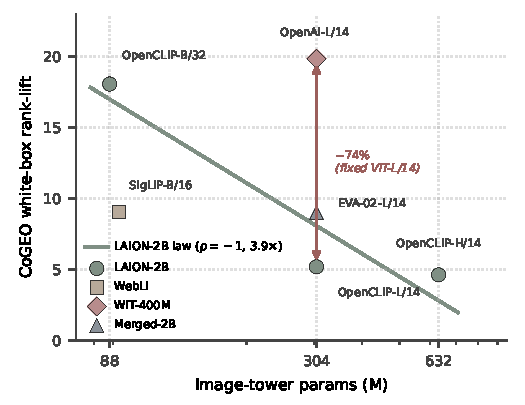
\includegraphics[width=0.82\columnwidth]{figures/fig_capacity_scaling.pdf}
\caption{Retriever capacity compresses the manipulable band. CoGEO white-box mean rank-lift (ESCI-491, $\eps = 16/255$, $224 \times 224$, product-title anchor; Fig.~\ref{M-fig:results}(e) of the main paper) versus image-tower parameter count (published model-card values, log scale). Within the corpus-controlled LAION-2B family (circles) the band contracts monotonically with capacity (Spearman $\rho = -1.0$, $\approx 3.9\times$); markers for the other pretraining corpora (OpenAI WIT-400M, EVA merged-2B, WebLI) show that a larger or cleaner pretraining corpus compresses the band further at fixed capacity (e.g.\ $-74\%$ from OpenAI to LAION-2B at ViT-L/14).}
\Description{Scatter of CoGEO white-box rank-lift against retriever image-tower parameters on a logarithmic x-axis, with the three LAION-2B points joined by a downward trend line and the other-corpus points marked separately; rank-lift decreases as capacity and pretraining-corpus quality increase.}
\label{sm:fig:capacity-scaling}
\end{figure}

\section{Anchor-source heterogeneity across vision--language captioners}
\label{sm:anchor-source}

The six-backbone replication (\S\ref{sm:cross-backbone}) varies the retriever while holding the anchor at the product title. To check robustness to the anchor source itself, we run CoGEO against the same six retrievers with five distinct vision--language captioners~\cite{li2022blip,li2023blip2,liu2024llava,wang2024qwen2vl,bai2024qwen25vl}, yielding a $5 \times 6 = 30$-cell ablation matrix on the same manifest.

\begin{figure}[t]
\centering
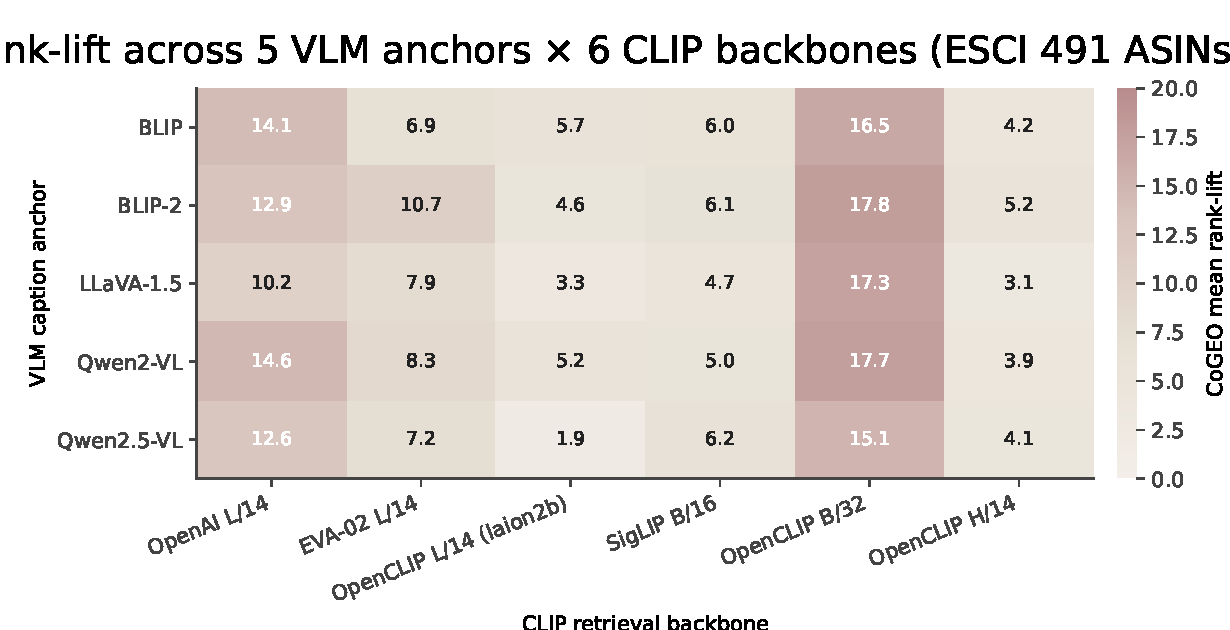
\includegraphics[width=0.95\columnwidth]{figures/fig_d_heatmap.pdf}
\caption{CoGEO mean rank-lift across $5$ vision--language captioner anchors $\times\ 6$ CLIP retrieval backbones on the $491$-ASIN ESCI manifest at $\eps = 16/255$, $224 \times 224$. Each row is one VLM caption source feeding the same CoGEO loop; each column is one CLIP retriever evaluating the resulting adversarial image. The backbone-axis range ($1.87$ on OpenCLIP-laion2b with Qwen2.5-VL captions to $17.79$ on OpenCLIP-B/32 with BLIP-2 captions) is roughly $4\times$ the within-column anchor-axis range, indicating that the retriever choice dominates the anchor choice.}
\Description{Five-by-six heatmap with vision--language captioners as rows (BLIP, BLIP-2, LLaVA-1.5, Qwen2-VL, Qwen2.5-VL) and six CLIP retrievers as columns. Column-wise color variation is much stronger than row-wise variation, indicating the retriever explains most of the rank-lift spread.}
\label{sm:fig:d-heatmap}
\end{figure}

\paragraph{Backbone dominates anchor} Within each row, the rank-lift spread across the six backbones is large ($\Delta \approx 11$--$13$). Within each column, the spread across the five anchor captioners is much smaller ($\Delta \approx 2$--$4$). The retriever choice therefore explains the bulk of CoGEO's effect; the anchor source is a secondary residual --- the operational form of an anchor-decoupled protocol surfacing the encoder-side property rather than a captioner artifact.

\paragraph{No anchor captioner is uniformly dominant} Per-column winners change (BLIP, Qwen2-VL, BLIP-2 each take some columns), and the within-column gap between best and worst captioner is under $5$ rank positions. A claim that depended on a specific captioner anchor would not be robust: the invariant of the main paper~\eqref{M-eq:invariant} --- any function of $x_p$ alone may serve as the anchor --- is borne out by the modest within-column variance.

\paragraph{Backbone-dependent attackability replicates with VLM anchors} The column-wise ordering (OpenCLIP-B/32 $\gg$ OpenAI L/14 $>$ EVA-02 $\approx$ SigLIP $\approx$ OpenCLIP-laion2b $\approx$ OpenCLIP-H/14) is preserved across all five anchor captioners: the property controlling how much CoGEO can move the ranking is the embedding, not the seller-side description.

\section{Perturbation-budget sensitivity}
\label{sm:eps_sweep}

The headline budget $\eps = 16/255$ is the value used in the main four-way comparison. Defenders care about the regime where attackers might prefer smaller, less perceptible perturbations~\cite{kurakin2017physical,wang2004ssim}. We sweep $\eps \in \{4, 8, 16\}/255$ on the same ESCI manifest with the OpenAI ViT-L/14 retriever for all four attacks; an earlier version of this sweep reported only CoGEO and the strongest baseline PGD-bare, and we now add AdvCLIP and Co-Attack so the budget-sensitivity claim is not restricted to the two leaders.

\begin{table}[t]
\centering
\caption{Perturbation-budget sweep on the ESCI $491$-image manifest with OpenAI ViT-L/14 at $224 \times 224$, now covering all four attacks. The $\eps = 16/255$ row is the four-way headline of the main paper (Table~\ref{M-tab:main4way}, $n = 560$); the $\eps \in \{4, 8\}/255$ rows use the $n = 500$ sweep subset. CoGEO, PGD-bare, and AdvCLIP strengthen with the budget; CoGEO's advantage over PGD-bare grows with $\eps$ and reverses only at the smallest budget.}
\label{sm:tab:eps-sweep}
\small
\setlength{\tabcolsep}{4pt}
\begin{tabular}{lrrrr}
\toprule
$\eps / 255$ & CoGEO & PGD-bare & AdvCLIP & Co-Attack \\
\midrule
\phantom{0}4 & ~8.50 & \textbf{~9.14} & $-0.75$ & ~3.34 \\
\phantom{0}8 & \textbf{12.20} & ~8.85 & ~1.78 & ~9.80 \\
16 & \textbf{19.86} & 12.37 & ~6.45 & ~5.77 \\
\bottomrule
\end{tabular}
\end{table}

\begin{figure}[t]
\centering
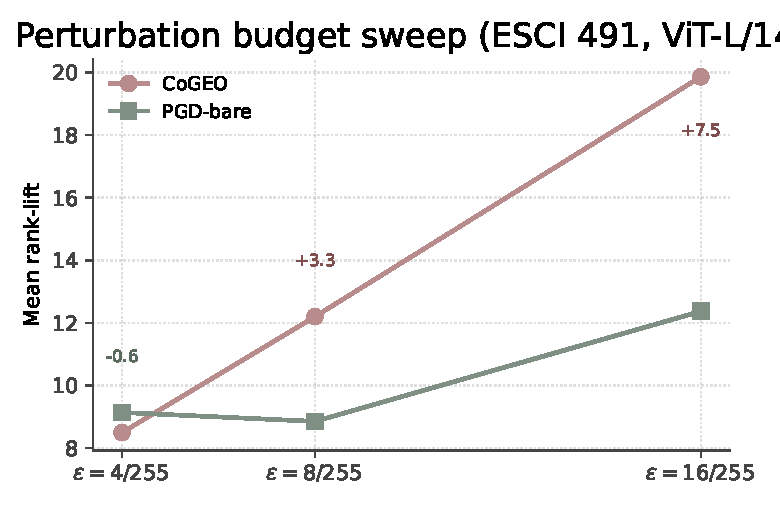
\includegraphics[width=\columnwidth]{figures/fig_eps_sweep_curve.pdf}
\caption{Mean rank-lift versus $L_\infty$ budget $\eps$ for CoGEO and PGD-bare on ESCI ($491$ ASINs, OpenAI ViT-L/14). CoGEO's margin over PGD-bare grows monotonically with the budget ($-0.64$, $+3.35$, $+7.49$ at $\eps = 4, 8, 16/255$) and reverses sign at the smallest budget.}
\Description{Line chart with two curves over three budgets 4/255, 8/255, and 16/255. CoGEO's curve rises steeply with the budget while PGD-bare's rises slowly; the curves cross near the smallest budget, where PGD-bare is slightly higher.}
\label{sm:fig:eps_sweep}
\end{figure}

Figure~\ref{sm:fig:eps_sweep} plots the rank-lift-versus-$\eps$ curve and Table~\ref{sm:tab:eps-sweep} records the exact values; the paragraphs below give the per-regime mechanism that the main paper abbreviates.

The sweep introduces a regime-dependent finding that a fixed-budget comparison does not surface.

\paragraph{Sub-budget regime: CoGEO can underperform PGD-bare} At $\eps = 4/255$, the headline conclusion of the main paper no longer holds: CoGEO underperforms PGD-bare by $0.64$ rank-lift on the same manifest. The likely mechanism is that CoGEO's auxiliary objectives---the differentiable JPEG layer~\cite{shin2017diffjpeg}, input diversity~\cite{xie2019dim,lin2020sim}, and Sobel-mask gradient gating---introduce regularization that consumes a fixed fraction of the gradient budget. At $\eps = 4/255$ that fraction is large enough relative to the effective signed step that PGD-bare's unmodified MI-FGSM~\cite{dong2018mifgsm,madry2018pgd} signal allocates more of the budget to direct anchor alignment.

\paragraph{Mid- and full-budget regime: monotone separation} As $\eps$ doubles to $8/255$ and again to $16/255$, CoGEO's advantage swings positive and grows monotonically: $+3.35$ at $\eps = 8/255$ and $+7.49$ at $\eps = 16/255$. The per-step regularizers stop being a bottleneck once the available perturbation budget is large enough to support a full anchor-aligned descent direction \emph{and} the diversity transforms~\cite{xie2019dim,lin2020sim}. The crossover happens between $\eps = 4/255$ and $\eps = 8/255$.

\paragraph{The two added attacks confirm the budget-monotone pattern} Extending the sweep to AdvCLIP and Co-Attack shows that both also strengthen with the budget rather than contradicting the headline: AdvCLIP rises monotonically $-0.75 \to 1.78 \to 6.45$, and Co-Attack rises $3.34 \to 9.80$ from $\eps = 4/255$ to $8/255$. Co-Attack is the one method whose $491$-set value does not increase from $\eps = 8/255$ to the $n = 560$ headline budget ($9.80$ vs $5.77$, measured on a smaller paired subset); on the $3\times$ larger $1{,}430$-pair sample of Section~\ref{sm:esci-scaleup} Co-Attack reaches $34.05$, so its low-headline figure is a sample-size effect rather than a true reversal. At the headline budget the four-way order is CoGEO $>$ PGD-bare $>$ AdvCLIP $\approx$ Co-Attack, and the low-budget crossover where PGD-bare edges CoGEO is specific to that pair, not an artifact of having compared only those two methods.

\paragraph{Refined statement of C3} Our main-paper C3 statement was a stealth--lift trade-off across methods at fixed $\eps$. The sweep adds a second axis: even within CoGEO, the trade-off shifts with $\eps$. A defender designing perceptual filters around an assumed $\eps = 16/255$ adversary therefore cannot extrapolate either the rank-lift or the SSIM~\cite{wang2004ssim} ranking to a smaller-budget adversary; the protocol of the main paper must be re-run with the budget the defender expects.

\section{A fifth attack family: a diffusion-prior generative attack}
\label{sm:diffprior}

The four-attack shortlist of the main paper covers per-image gradient, universal-patch, and cross-modal families, and the limitations list a diffusion-prior attack among the unmeasured families. We close that gap with a fifth family: a latent-diffusion generative attack~\cite{rombach2022ldm} that synthesizes an anchor-aligned perturbation through a Stable-Diffusion prior rather than by direct signed-gradient ascent. We generate the diffusion-prior perturbation for all $491$ manifest images and re-score it on the OpenAI ViT-L/14 white-box surrogate with the identical evaluation harness used for the four headline families ($n = 500$ held-out shopper-query pairs, $L_\infty$ budget $\eps = 16/255$).

\begin{table}[t]
\centering
\caption{Five-family comparison on the OpenAI ViT-L/14 white-box surrogate ($n = 500$ held-out ESCI shopper-query pairs, $\eps = 16/255$), re-scored with the headline evaluation harness. Rank-lift is the mean positions an image rises against its held-out query; higher is a stronger attack. The diffusion-prior family is added to the four families of the main paper.}
\label{sm:tab:diffprior}
\small
\begin{tabular}{lc}
\toprule
Attack family & Mean rank-lift \\
\midrule
CoGEO & \textbf{15.60} \\
PGD-bare & 13.58 \\
Diffusion-prior~\cite{rombach2022ldm} & 13.18 \\
Co-Attack & 12.82 \\
AdvCLIP & 5.06 \\
\bottomrule
\end{tabular}
\end{table}

\paragraph{The diffusion-prior attack is mid-pack and does not overtake CoGEO} On the common surrogate the five families order as CoGEO $15.60 >$ PGD-bare $13.58 \approx$ diffusion-prior $13.18 \approx$ Co-Attack $12.82 \gg$ AdvCLIP $5.06$ in mean rank-lift (Table~\ref{sm:tab:diffprior}); the median rank-lift is $1$ for every family except AdvCLIP ($0$), matching the heavy-right-tail pattern of the main paper. The diffusion-prior attack thus sits squarely among the gradient baselines --- comparable to PGD-bare and Co-Attack, far above the universal patch --- but stays decisively below the anchor-decoupled CoGEO loop, and its held-out CLIP-similarity gain ($0.0342$) and Irrelevant$\to$top-$3$ promotion ($9.1\% \to 14\%$ against the unperturbed $9.1\%$ baseline) are likewise in the baseline band. To confirm the fifth number is comparable to the headline roster rather than an artifact of a separate run, the same re-scoring pass reproduces the published per-method values of the two reference attacks (CoGEO $15.60$ vs.\ published $15.7$--$16.0$; PGD-bare $13.58$ vs.\ $13.6$), so the surrogate and harness match.

\paragraph{Implication} The result strengthens rather than weakens the recalibration. A generative diffusion prior --- a perturbation mechanism structurally different from signed-gradient ascent --- reaches only the strong-baseline band and does not beat CoGEO's anchor-alignment objective, so the main paper's top-$1$ ordering is not an artifact of having compared against gradient attacks alone. It also closes the self-declared diffusion-prior gap in the limitations, leaving evolutionary search as the remaining unmeasured family.

\section{Evaluation-pass and CoGEO inner-loop pseudocode}
\label{sm:cogeo-pseudocode}

This section gives the two pieces of pseudocode referenced from the main-paper method section (Section~\ref{M-sec:method}). Algorithm~\ref{alg:protocol} is the anchor-decoupled evaluation pass run once per attack family: it makes the anchor$\perp$query invariant verifiable line by line, because the cohort label $\ell_i$ enters only the per-cohort decomposition while the held-out query $q_i$ enters only the rank-lift and held-out cosine measurements and is never passed to the attack $\mathcal{A}$.

\begin{algorithm}[t]
\caption{Anchor-decoupled evaluation pass (per attack family).}
\label{alg:protocol}
\small
\begin{algorithmic}[1]
\Require ESCI triples $\mathcal{D}=\{(q_i, x_{p,i}, \ell_i)\}_{i=1}^{N}$, retriever $(E_I, E_T)$, attack $\mathcal{A}$, budget $\eps$
\State \textbf{Pre-flight gate:}\ compute mean cosines per cohort using $E_I$ and $E_T$ at no perturbation
\State \quad \textbf{require} $\overline{\cos}_{\ell=E} - \overline{\cos}_{\ell=I} \geq 0.05$; \textbf{else swap backbone and restart}
\For{each $(q_i, x_{p,i}, \ell_i) \in \mathcal{D}$}
  \State $v_{\mathrm{anchor}}(x_{p,i}) \gets E_T(\textsc{SellerAnchor}(x_{p,i}))$
        \Comment{depends only on $x_p$}
  \State $\delta_i \gets \mathcal{A}(x_{p,i},\ v_{\mathrm{anchor}}(x_{p,i}),\ \eps)$
        \Comment{$q_i$ is \emph{not} passed to $\mathcal{A}$}
  \State $x_{p,i}^* \gets \text{clip}(x_{p,i} + \delta_i,\,[0,1])$
  \State $r_i \gets \text{rank}(x_{p,i}^*,\ q_i;\ \text{candidate pool}) - \text{rank}(x_{p,i},\ q_i;\ \cdot)$
  \State $s_i \gets \cos(E_I(x_{p,i}^*),\,E_T(q_i)) - \cos(E_I(x_{p,i}),\,E_T(q_i))$
  \State $\sigma_i \gets \mathrm{SSIM}(x_{p,i}^*,\,x_{p,i})$ at $224\times 224$
\EndFor
\State \textbf{Decompose} $\{r_i\}$ and $\{s_i\}$ by cohort label $\ell\in\{E,S,C,I\}$
\State \textbf{Significance:} report paired Wilcoxon signed-rank~\cite{wilcoxon1945individual} $p$-values for each method pair, plus paired bootstrap $95\%$ CIs
\State \Return aggregate and per-cohort statistics for $\mathcal{A}$
\end{algorithmic}
\end{algorithm}

The CoGEO inner loop invoked from that pass is fully specified by the masked MI-FGSM update of the main-paper method section. Algorithm~\ref{alg:cogeo} restates it in step-by-step pseudocode for reference; it is identical to the equations in the main text and introduces no additional hyperparameters.

\begin{algorithm}[t]
\caption{CoGEO inner loop (one of the four attack families in the anchor-decoupled evaluation pass).}
\label{alg:cogeo}
\small
\begin{algorithmic}[1]
\Require image $x_p$, anchor $v_{\mathrm{anchor}}$, budget $\eps$, step $\alpha$, iterations $T$, momentum $\mu$, JPEG quality $Q$
\State $M \gets \textsc{SobelMask}(x_p, \tau)$ \Comment{high-gradient region only}
\State $\delta \gets \mathbf{0}$,\quad $g \gets \mathbf{0}$
\For{$t = 1$ to $T$}
  \State $\tilde{x} \gets \textsc{DiffJPEG}(x_p + \delta;\ Q)$
  \State $L \gets -\,\cos\bigl(E_I(\tilde{x}),\ v_{\mathrm{anchor}}\bigr)$
  \State $g \gets \mu \cdot g + \nabla_{\delta} L\,/\,\lVert \nabla_{\delta} L\rVert_1$
  \State $\delta \gets \delta - \alpha \cdot M \odot \mathrm{sign}(g)$
  \State $\delta \gets \mathrm{clip}_\infty(\delta,\,-\eps,\,+\eps)$
  \State $\delta \gets \mathrm{clip}(x_p + \delta,\,0,\,1) - x_p$
\EndFor
\State \Return $\delta$
\end{algorithmic}
\end{algorithm}

